\documentclass[handout]{beamer}
%\documentclass [serif,mathserif,professionalfont]{beamer}
%\usepackage {pxfonts}
%\usepackage {eulervm}
%\usepackage{mathpazo}
%\logo{\includegraphics[height=1.2cm]{fsulogo.png}}

\usepackage{tikz}
\usepackage{graphicx}
\usepackage{subfig,fixltx2e,url}
\usepackage[latin1]{inputenc}
\usepackage{pgfplots}
\usepackage{hyperref}
\usepackage{booktabs}

%\usetheme{Warsaw}
\usecolortheme{lily}
\setbeamercovered{transparent}
%\useoutertheme[subsection=false]{smoothbars}

\setbeamertemplate{sidebar right}{}
\setbeamertemplate{footline}{%
\hfill\usebeamertemplate***{navigation symbols}
\hspace{1cm}\insertframenumber{}/\inserttotalframenumber}

\title[ \insertdate]{Multi-Input Multi-Output Electric Motor Signal Prediction using Neural Networks}

\author{Sagar Verma}
\institute[Centralesup\'elec and Schneider Electric] % (optional, but mostly needed)
{
  Centre de Vision Num\'erique,\\
  Centralesup\'elec, Gif-sur-Yvette}
% - Use the \inst command only if there are several affiliations.
% - Keep it simple, no one is interested in your street address.

\date{December, 2018}
% - Either use conference name or its abbreviation.
% - Not really informative to the audience, more for people (including

\begin{document}

\begin{frame}
\titlepage
\end{frame}

\begin{frame}{Table Of Contents}
\begin{enumerate}
\item Dataset
\item Experiments
\item Results
\item Questions
\end{enumerate}
\end{frame}

\section{Problem Statement}

\begin{frame}{What we discussed in the last meeting?}
\begin{enumerate}
  \item Problem definition
  \item Neural networks introduction
  \item Early results on public dataset
  \item Error in predicting impulse peeks
  \item Prediction scaling problem
\end{enumerate}
\end{frame}


\begin{frame}{Dataset}{Description}
  \begin{enumerate}
    \item Single experiment
    \item 1200 seconds long
    \item Simulink dq-frame model is used
  \end{enumerate}
\end{frame}

\begin{frame}{Dataset}{Voltages}
\begin{center}
  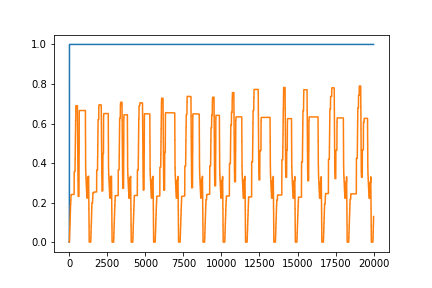
\includegraphics[width=0.8\linewidth, height=4cm]{images/voltages}
\end{center}
\end{frame}

\begin{frame}{Dataset}{Stator Pulse}
\begin{center}
  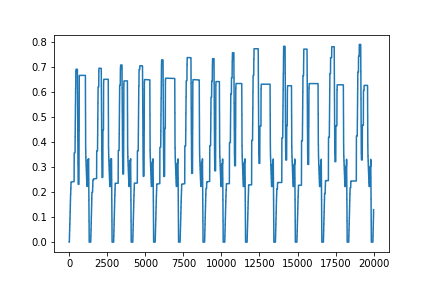
\includegraphics[width=0.8\linewidth, height=4cm]{images/stator_pulse}
\end{center}
\end{frame}

\begin{frame}{Dataset}{Speed}
\begin{center}
  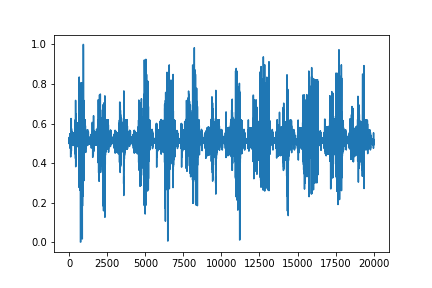
\includegraphics[width=0.8\linewidth, height=4cm]{images/speed}
\end{center}
\end{frame}

\begin{frame}{Dataset}{Currents}
\begin{center}
  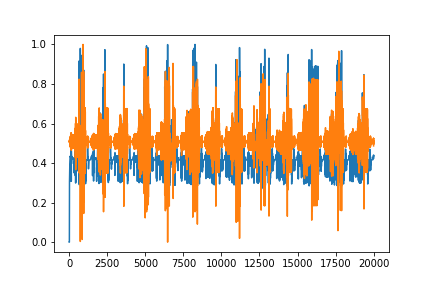
\includegraphics[width=0.8\linewidth, height=4cm]{images/current}
\end{center}
\end{frame}

\begin{frame}{Dataset}{Torque}
\begin{center}
  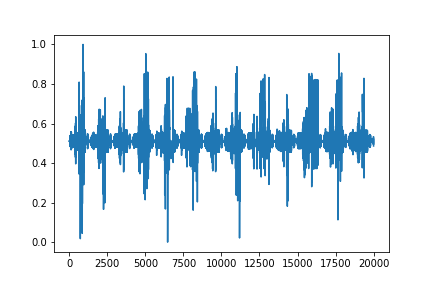
\includegraphics[width=0.8\linewidth, height=4cm]{images/torque}
\end{center}
\end{frame}

\begin{frame}{Dataset}{Voltage2 and Stator Pulse}
\begin{center}
  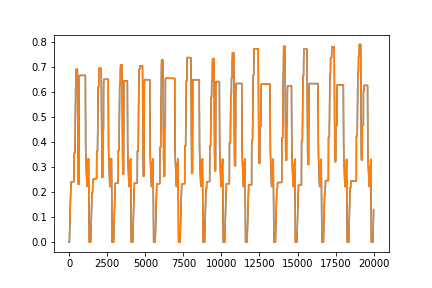
\includegraphics[width=0.8\linewidth, height=4cm]{images/voltage2_stator_pulse}
\end{center}
\end{frame}

\begin{frame}{Dataset}{Train-Test Split}
  \begin{enumerate}
    \item Single experiment
    \item Biased if the split is 0-800s and 800-1200s
    \item Random sampling
      \begin{enumerate}
        \item Take window $w$ with stride $s$
        \item Randomply sample windows
        \item Train-test cover whole data
        \item No overlaping b/w train-test
      \end{enumerate}
  \end{enumerate}
\end{frame}

\begin{frame}{Experiments}{Input selection}
  \begin{enumerate}
    \item Use simulking for downsampling
    \item Stride $s$ = 1,5,10; Works best at stride 1
    \item Windows sizes that matter, $5\leq w<10$ and $10\leq w \leq100$
    \item Ignore voltage 1
    \item Use either voltage 2 or stator pulse
  \end{enumerate}
\end{frame}

\begin{frame}{Experiments}{Output selection}
  \begin{enumerate}
    \item Don't predict all time steps
    \item Predict first, middle or last time step
    \item Middle works better
  \end{enumerate}
\end{frame}

\begin{frame}{Experiments}{ANN for signal prediction}
  \begin{enumerate}
    \item Three outputs, three networks.
    \item Input: $w\times3$ 1-D vector, Output: $1$ middle value
    \item Activation, $f$: Leaky Relu
  \end{enumerate}
  \begin{center}
    \begin{figure}
    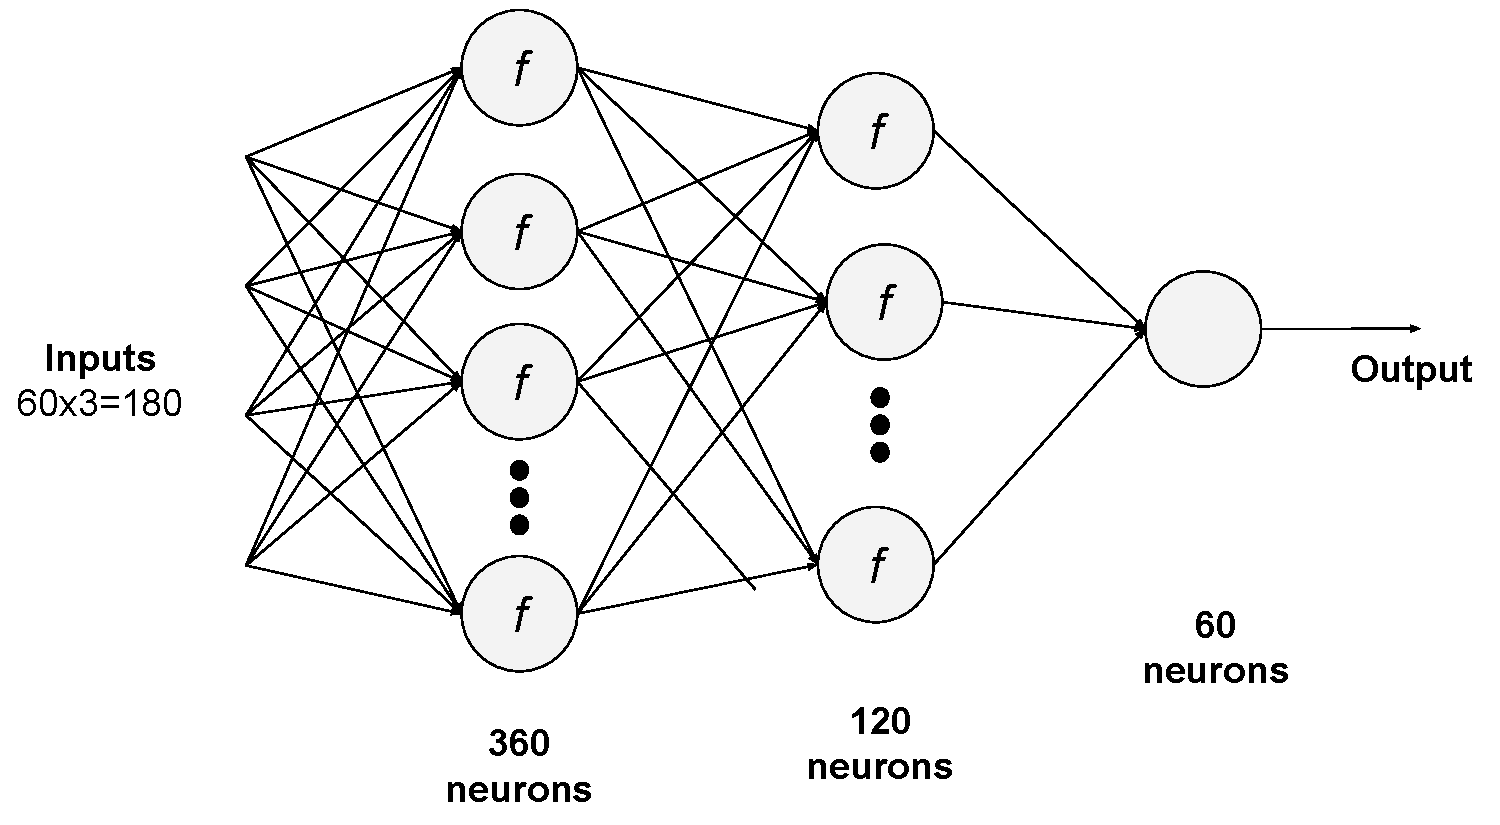
\includegraphics[scale=0.35]{images/motor_ann_1}
    \end{figure}
  \end{center}
\end{frame}

\begin{frame}{Experiments}{ANN with auxiliary task}
  \begin{enumerate}
    \item Also reconstruct input signal.
    \item Three outputs, three networks.
    \item Input: $w\times3$ 2-D vector, Output1: $1$, output2: $w\times3$ 2-D vector
    \item Activation, $f$: Leaky Relu
  \end{enumerate}
  \begin{center}
    \begin{figure}
    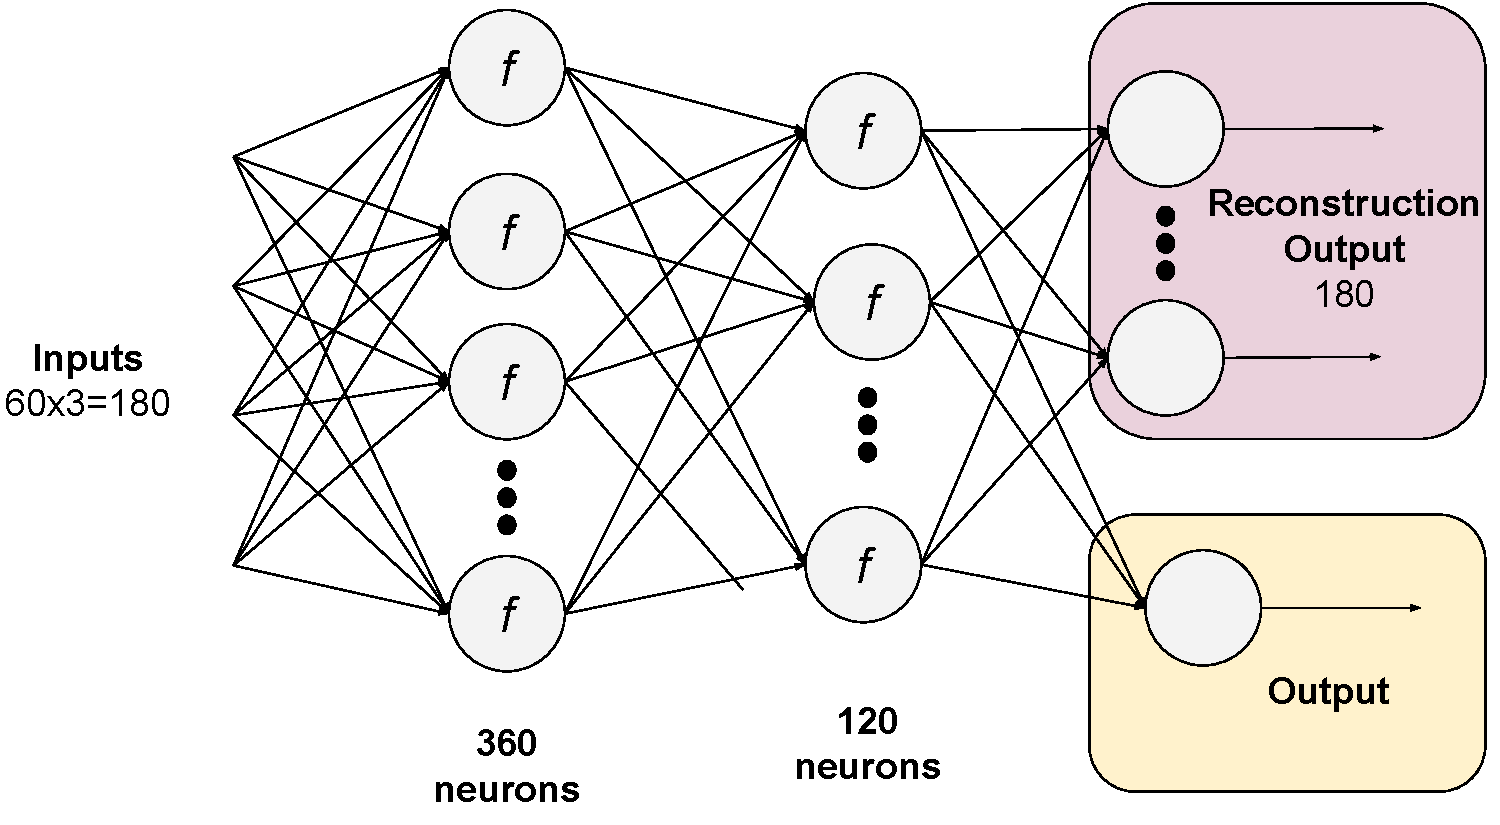
\includegraphics[scale=0.35]{images/motor_recon}
    \end{figure}
  \end{center}
\end{frame}

\begin{frame}{Experiments}{Convolution network}
  \begin{enumerate}
    \item CNN and ANN works better then RNN (Miller et al. 2018).
    \item Kernels capture $w\leq10$
    \item Channel featurization, correlate voltage2 and speed
    \item Three outputs, three networks.
    \item Input: $w\times3$ 2-D vector, Output: $1$
    \item Activation, $f$: Leaky Relu (in conv)
  \end{enumerate}
  \begin{center}
    \begin{figure}
    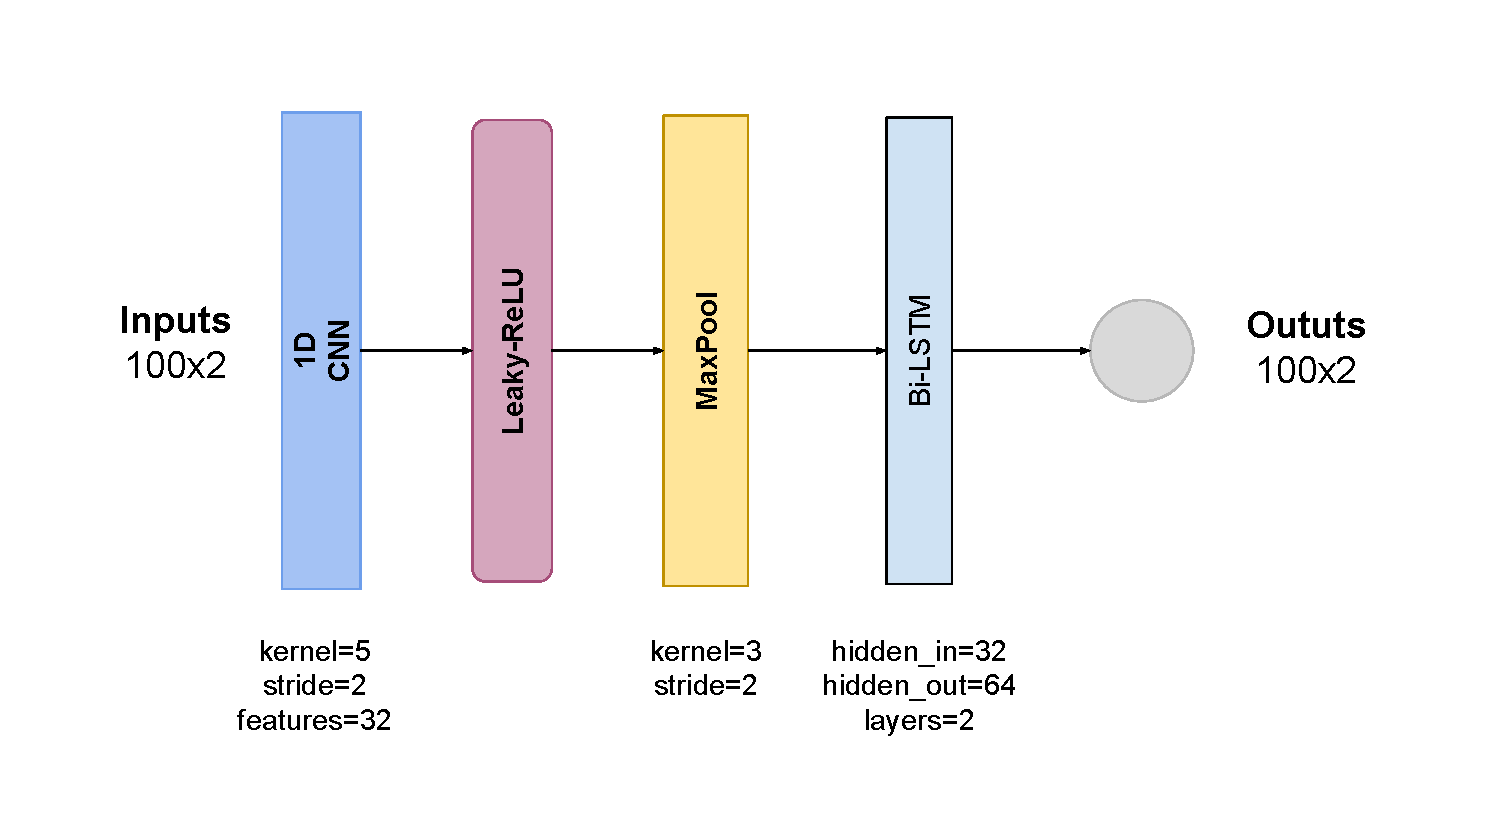
\includegraphics[scale=0.35]{images/motor_cnn}
    \end{figure}
  \end{center}
\end{frame}


\begin{frame}{Results}{Best Model}
\begin{table}[]
  \begin{tabular}{l c c c c}
  \toprule[0.2mm]
   \textbf{Model} & \textbf{w} & \textbf{Current1} & \textbf{Current2} & \textbf{Torque}\\
   \midrule
   \textbf{ANN} & 100 & 0.223 & 0.197 & 0.101 \\
   \midrule
   \textbf{ANN Aux} & 100 & 0.192 & 0.182 & 0.112 \\
   \midrule
   \textbf{CNN} & 100 & \textbf{0.107} & \textbf{0.104} & \textbf{0.091} \\
   \bottomrule
  \end{tabular}
  \caption{MSE of different models.}
  \end{table}
\end{frame}
% \begin{frame}{RBM for signal prediction}
%
% \end{frame}

\begin{frame}{Results}{Example Outputs}
\begin{center}
  \begin{figure}
  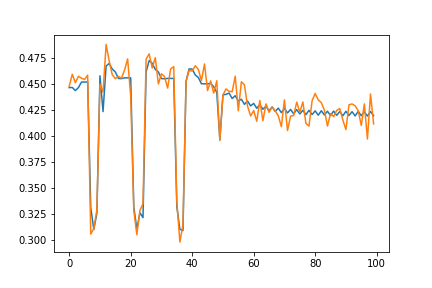
\includegraphics[scale=0.25]{images/plot_current1}
  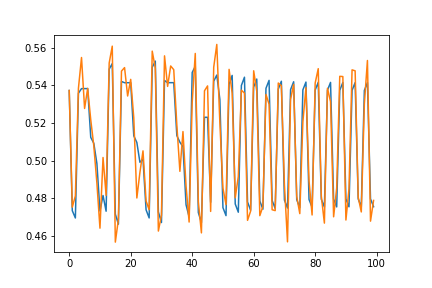
\includegraphics[scale=0.25]{images/plot_current2}
  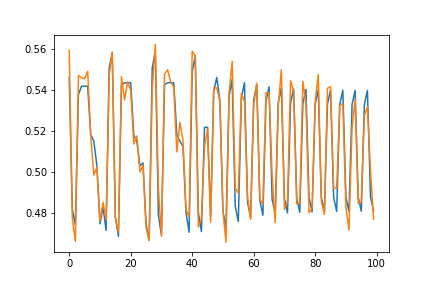
\includegraphics[scale=0.25]{images/plot_torque}
  \center{\caption{Left to right: current1, current2, and torque, orange color: predicted}}
  \end{figure}
\end{center}
\end{frame}

\section{Questions}
\begin{frame}{Questions}
\begin{enumerate}
  \item Is data very simple?
  \item When voltage 1 is not constant?
  \item When Voltage 2 and stator pulse are not same?
  \item Can signals be grouped into some classes?
  \item Visual evaluations?
  \item Other evaluation metrics?
  \item Predict future(causal)?
\end{enumerate}
\end{frame}

\begin{frame}
\center
\color{blue}
\huge{Thank you!}\\
\end{frame}

\end{document}
